\section{Results and Discussion}
\label{sec:res}
\subsection{Mean Asphericity and Critical Cumulant}

The main goal of this section is to learn how magnetic properties of Ising-like models depend on their geometrical ones and to determine their comparability in the critical region, where dependence of model observables from the length of conformation $N$ is the weakest. 
The idea is to compare critical cumulants $U_{4}$ \eqref{eq:Cumulant} of both models of Ising having equal asphericities. 
Both models are considered to have open boundary conditions (OBC). 
To the best of the author’s knowledge, in the Ising model on rectangular lattice shape factors like aspect ratio $r$ are the parameters, not observable values. 
Therefore, it became possible to find value of the aspect ratio of lattice for any asphericity $\mathcal{A}$ \eqref{eq:Asphericity} (see figure \ref{fig:A_r}). 
For rectangular lattice, the leading correction term to the asphericity behave like $A^{*}(r) - A(r, L) \propto 1 / L^{2}$. 
Moreover, the value of Binder cumulant in Rectangular Ising in critical region depends on aspect ratio $r$ \cite{Selke2006}.

\begin{figure}[h]
    \centering
    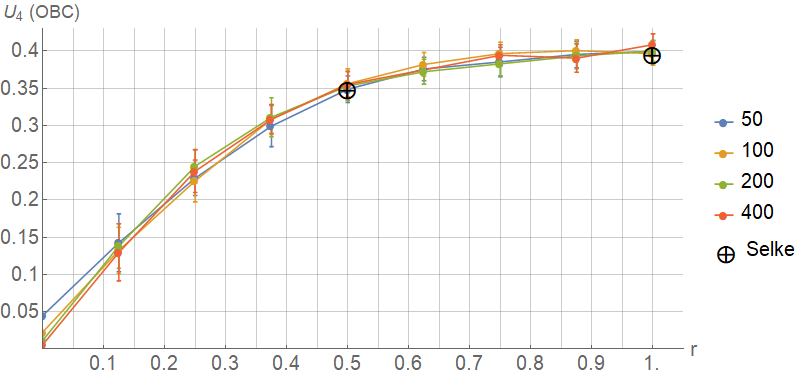
\includegraphics[width=0.5\textwidth]{Images/CumulantOBC.png}
    \caption{Critical cumulant $U_{4}$\eqref{eq:Cumulant} of Ising model on a rectangular lattice with open boundary conditions as function of aspect ratio $r$ with side length $L$ = 50 (blue), 100 (yellow), 200 (green) and 400 (red). Black markers define values from \cite{Selke2006}}
    \label{fig:A_r}
\end{figure} 

By performing Monte-Carlo simulations with steps of Wolff algorithm \cite{Newmanb1999} on Ising model on a rectangular lattice with open boundary conditions in $\theta$-point ($J_{c} = \ln{(1 + \sqrt{2}) / 2} =  0.44068... $), the statistics for Binder cumulant $U_{4}$ were collected with respect to aspect ratio $r$ (see \cref{tab:Ising_T_c}). The results matched with known values from \cite{Selke2006}.

\begin{figure}[h]
    \centering
    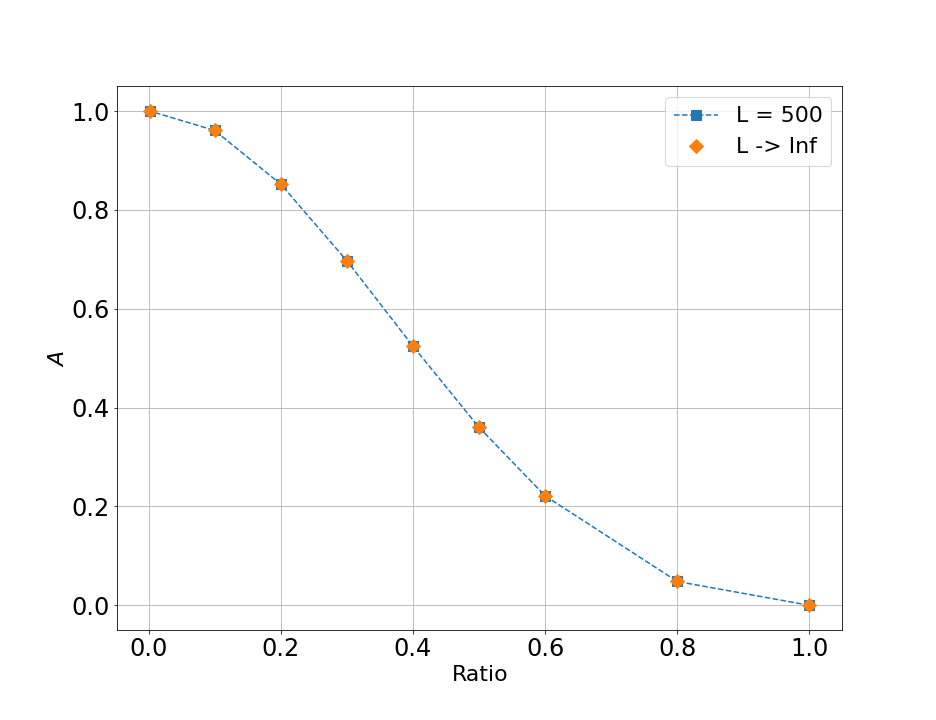
\includegraphics[width=0.5\textwidth]{Images/A_r.png}
    \caption{Asphericity as function of aspect ratio $r$ of the rectangular lattice with side length = 500 and approximate values for rectangular lattice with infinitely long side}
    \label{fig:A_r}
\end{figure}


Ising-ISAW and ISAW models were also simulated on the 2D-square lattice for lengths N = 1000-4900 with the algorithm described in \cite{faizullina2021critical}. 
The simulations were performed for $0 < J < 1$, focusing on areas near the respective critical regions.

\Cref{fig:Ising&ISAW_A_J} shows results of the simulations for asphericity \eqref{eq:Asphericity} as function of J. 
For ISAW model $J_{c} = 0.6673(5)$, and the results are matching to known values from \cite{Caracciolo2011}, where critical region was also enumerated.
A critical value of Ising-ISAW model was took from previous work: $J_{c} = 0.8340(5)$ \cite{faizullina2021critical}, while the border critical values depicts results from \cite{Foster2021} ($J_{c} = 0.8340 \pm 0.0021$). 
Both values were marked as black vertical lines with blue zone around, which will be referred to as all statistical errors of critical regions. 
The figure \ref{fig:Ising&ISAW_A_J} depicts that the results for ISAW model in this paper are agreed with the value of critical asphericity of ISAW model from \cite{Caracciolo2011} defined with the horizontal line.

\begin{figure}[h!]
        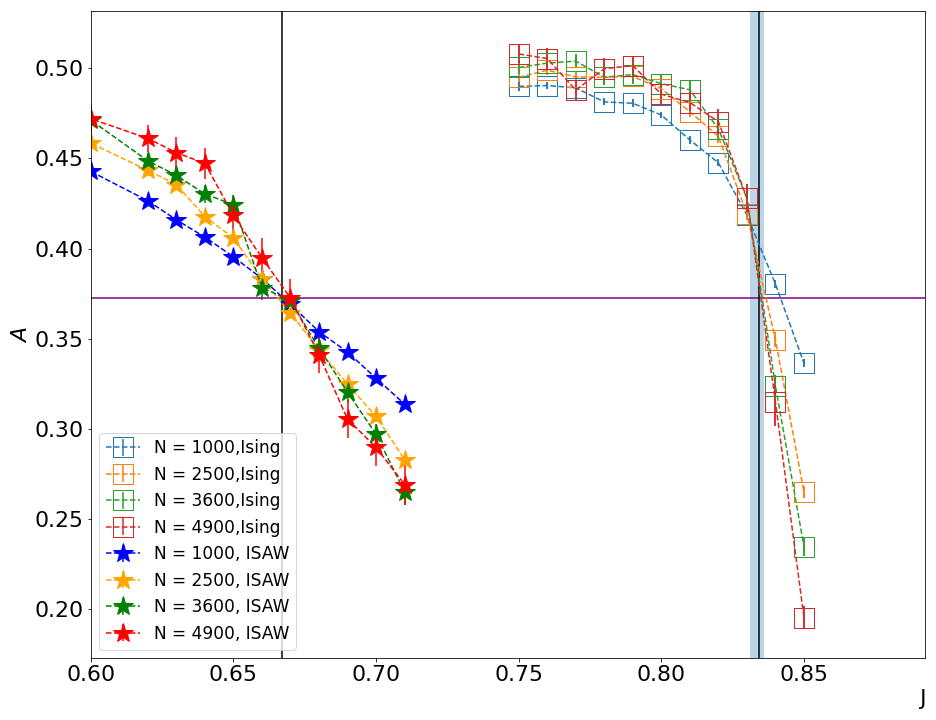
\includegraphics[width=0.5\textwidth]{Images/Ising_ISAW_A_J_Full.png}
        \caption{Asphericity of Ising-ISAW (empty squares) and ISAW-only models (stars) as function of $J=1/T$, varying lengths of conformations $N$ = 1000 (blue), 2500 (yellow), 3600 (green) and 4900 (red)}
        \label{fig:Ising&ISAW_A_J}
\end{figure}
\begin{figure}[h!]
        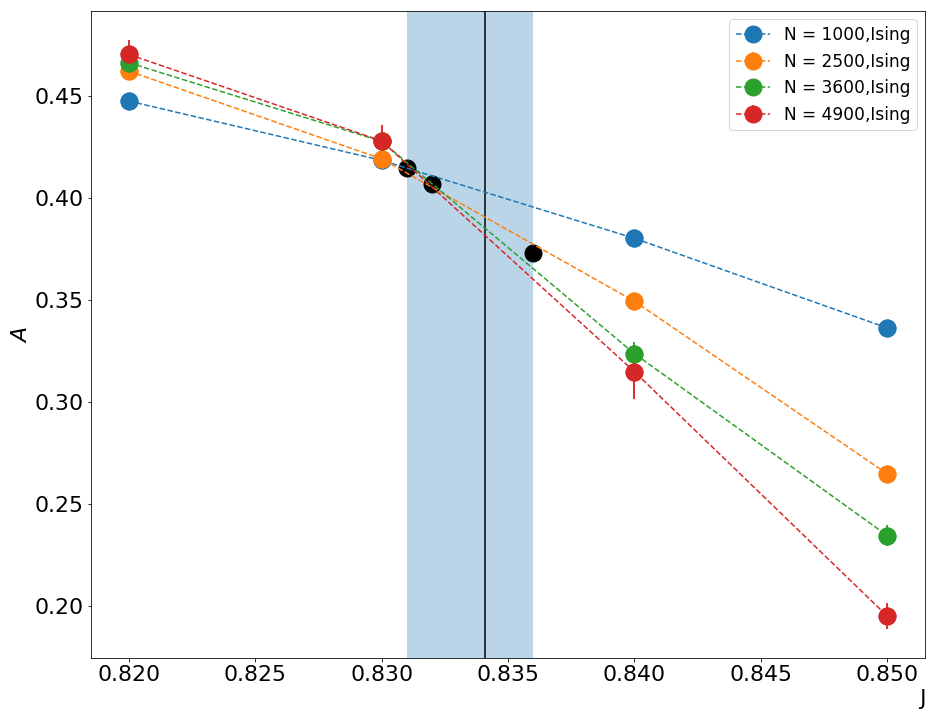
\includegraphics[width=0.5\textwidth]{Images/Ising_A_J_Close.png}
        \caption{Asphericity of Ising-ISAW model as function of zoomed in the critical region (blue zone, according to \cite{Foster2021} and black vertical line, according to \cite{faizullina2021critical}), varying lengths of conformations N = 1000 (blue), 2500 (yellow), 3600 (green) and 4900 (red)}
        \label{fig:Ising_A_J}
\end{figure}


The mean values of asphericity of Ising-ISAW model were took in the borders of critical region and in the point of the best crossing of plots where phase transition can be observed according to the previous numerical results. 
All these points are marked as black in zoomed figures \ref{fig:Ising_A_J}. 
The following steps were to pick up values of aspect ratio, to perform simulations of the Rectangular Ising with the same ratio and, consequently, asphericity and to find critical cumulant of the model with the same shape factors. 
As figure \ref{fig:A_r} depicts, it is enough to use lattice with length $N$ = 500 for picking up the aspect ratio. 
Simulations were performed with the use of the cluster update based on Wolff algorithm \cite{Newmanb1999} on a rectangular lattice with the same length.\\

\begin{table}[h]
    \centering
    \begin{tabular}{|c|c|c|c|}
        \hline
         \multicolumn{4}{|c|}{Ising-ISAW}  \\ \hline
         J & $\mathcal{A}$ & r & $U_{4}\  Rectangular$ \\ \hline
         0.831 & 0.415 & 0.465 & $0.338 \pm 0.006$\\ \hline
         0.832 & 0.4072 & 0.47 & $0.343 \pm 0.006$\\ \hline
         0.836 & 0.373 & 0.492 & $0.349 \pm 0.006$\\ \hline
         \end{tabular}
    \medskip
    \caption{Values of critical cumulant for Ising model on rectangular lattice with mean asphericity related to Ising-ISAW model in its critical region}
    \label{tab:A_r_U}
\end{table}


As a result, comparison with critical cumulant of Ising-ISAW model, which value was found during simulations in \cite{faizullina2021critical} ($U_{4} = 0.308(8)$) showed significant mismatch of values. 
It means that some other geometrical properties might have not been took into account properly - for example, which will be considered in the section \ref{sec:resB} - proportions of monomers with different quantities of nearest neighbors. 
It is obvious that in Ising model on the rectangular lattice most of monomers are located inside the lattice and have 4 nearest neighbors, while monomers spread around the perimeter of the lattice have only 2 (corners) or 3 nearest neighbors. The proportions in Ising-ISAW conformations are completely different (see figure \ref{fig:Ising_vs_ISAW2D}).



\subsection{Bulk}
\label{sec:resB}

The section discusssed the proportions of monomers with fixed numbers of nearest neighbors for Ising-ISAW and ISAW models on 3D-square and 2D-triangular lattices. 
Monomers of all four modified models can have from 2 to 6 close-range energy connections. 
Some types of monomers, according to the number of connections they have, can be interpreted similarly: for example, parts of conformations with monomers with only two nearest neighbors represent 1D-conformations or chains whatever lattice was used in observed model. 
And the opposite - regions where monomers have maximum number of close-range connections represent densely packed areas deep inside the globule. 
In the case of conformations on cubic lattice, other types of monomers can be also interpreted: monomers with only three neighbors define "corners" on conformation, while only monomers on a cube edge (or it also can be on a isolated plane from other part of globule) can have four neighbors. 
Presence of five neighbors belongs to the monomers on a surface of conformation. 
Unfortunately, the similar interpretations cannot be defined for conformations on a triangular lattices.

The first step was to perform simulations of ISAW model on square lattice on lengths from 5 to 3600 at $J=0$ with collecting statistics for fraction of monomers with 2 to 4 neighbors. 
To understand the mechanics of calculating neighbors of monomers, it is required to manually enumerate fractions of monomers with these number of neighbors for short conformations (5 to 11). 
The results of both methods are appeared to be the same.


\subsubsection{Ising model on a SAW-conformation}

Proportions of monomers with 2-6 nearest neighbors in Ising-ISAW model on a three-dimensional square (or cubic) lattice were simulated using method of MC simulations from \cite{faizullina2021critical}.

As it is seen from the left part of \Cref{fig:Ising_vs_ISAW}, increasing the strength of nearest-neighbors interaction J leads to conformation becoming more dense as proportions of monomers with higher numbers of close-range connections significantly increases after $\theta$-transition located in a blue zone (for Ising-ISAW model on a cubic lattice $T_{c} = 0.5263 \pm 0.055$\cite{Foster2021}) (see table \ref{tab:Ising_T_c}).

MC simulations were repeated for two-dimensional triangular lattice. 
Unlike the 3D-square lattice, the 5-th and 6-th possible neighbors located on the same plane as the first four, so conformations are expected to be more dense on this lattice.

The critical region of the model on a triangular lattice has not been enumerated yet. 
But as it was suggested, density of conformations becomes higher as nearest-neighbors interaction $J$ strengthen. 
Moreover, the proportion of monomers with six neighbors on a triangular lattice is far higher than on a cubic one. 
It is also significant that "triangular" conformations with no inner interaction have almost twice shorter one-dimensional chains than conformations on a cubic lattice in the same conditions.

\subsubsection{ISAW model}

To understand how the presence of magnetic properties affects the density of models, Monte-Carlo simulations were also performed on a parental model of the interacting self-avoiding walks on the same lattices. 
Results was similar to Ising-ISAW model, as suggested from "parent" model. 
For cubic lattice $T_{c} = 0.2779\pm 0.0041 $\cite{Tesi1996} while for triangular lattice $J_{c} = 0.405 \pm 0.07 $\cite{Privman1986}. 
\Cref{fig:Ising_vs_ISAW} shows that geometric aspects of phase transition in ISAW model manifect earlier than in Ising-ISAW ones.  



\section{Anticipated results}
\label{sec:antres}
Another attactive area of research is zero-interaction zone, where interaction strength J is close to zero and Ising-ISAW and ISAW models converts to non-interacting SAWs.
In previous work \cite{faizullina2021critical}, it was shown that the proportion of monomers with 3 neighbours of 2D-square Ising-ISAW model was close to a quarter in zero-interaction zone.
So the further goals of this work are to estimate the scaling nature of SAW models as functions of conformation length and the coefficients of scaling functions.
It is expected that the behaviour of triangular ISAW will be more close to cubic modification, than to 2D-square version. 
